\chapter{Introduction}

Since proteins are the base of a variety of roles such as acting as enzymes, transporting small molecules, forming cellular structures, regulating cell processes, carrying signals etc, understanding proteins would help in solving a number of unanswered questions which still elude biologists. A protein's primary structure consists of a linear combination of monomers (amino acids) of 20 different kinds. Under various physiological conditions, this linear arrangement folds and adopts a specific geometric pattern called the tertiary structure of the protein. Therefore, residues which are distant in the linear combination can come close to each other in this 3D structure forming a close bond (contact). It is this 3D structure of a protein that determines its macroscopic properties, behaviors and functions. Proteins that are similar in their structures will likely have similarity in functions. Quite naturally, studying the 3D structure of a protein has been an active area of research for the last two decades. This report looks into studying protein structure similarity by aligning a protein to the known structure of another protein. Before going into the details of {\it Protein Structure Similarity}, in the next two sections, some of the basic definitions are introduced that will be used through the rest of the report.

\section{Protein Structure Similarity}

The 3D structure of the protein has earlier been predicted from its amino acid sequence \emph{via} numerous experimental processes like X-ray crystallography \citep{anca08} or Nuclear Magnetic Resonance \cite{walc13} but efforts have also been made for designing computer algorithms to predict the same. This process of predicting the 3D structure of a protein from its amino acid sequence is called {\it Protein Folding Problem} \citep{bele98,crgp98,dima12}. However, even after significant research, the protein folding problem stays computationally intractable.
%Now a protein's amino acid sequence determines its 3D structure which in turn determines its functional propertie. So
An alternative approach to study the functional properties of a protein, perhaps computationally more tractable, is to find similarity of a given protein with other proteins.
%So another vast area of research developed on studying the protein structure similarity.
There could be two different types of similarity that one can study -- sequence similarity and structural similarity. Sequence similarity is a far less reliable method than structural similarity as it is the structure of the protein that determines its functional properties. To compute the similarity between two protein 3D structures, one needs some scoring mechanism that captures the biological relevance of the chemical and physical constraints involved in molecular recognition. Few such known and available structural similarity measures are listed below:
\begin{noindlist}
\item {\it Root Mean Square Division} (RMSD) -- measures root of sum of the squares of Euclidean distance between mapped residues \citep{cost80,diamond88,diamond92},
\item difference between the distance matrices \citep{hosa93,hosa96,huph04},
\item {\it Contact Map Overlap} (CMO)-- measures the pairwise distance between residues of each protein \citep{goip99,agmw07,anmy11},
\item \emph{ad-hoc} score based on local secondary structure, hydrogen bonding pattern or interaction environment \citep{bljo93,vrsa91,taor89,zuso89}.
\end{noindlist}

This report deals only with the {\it Contact Map Overlap} scoring scheme.
Of the various structures used to represent a protein, a simplified lattice model is adopted to
represent the backbone of the protein to study CMO.
The protein is represented as a non-self intersecting path on an integer grid in two or three dimensions, formally known as a self-avoiding walk. Details of such construction and assumption are described in the following sections.

\section{Contact and Contact Map Overlap (CMO)}
Since proteins are not just a collection of arbitrary edges, the structure of a protein is represented on the lattice using a {\it self-avoiding walk}. As the term suggests, a self-avoiding walk is a sequence of moves on the lattice that will not visit the same point twice, \emph{i.e.} a path from a point to another will never intersect itself.
%One should note that the emphasis is mostly on the contacts between sets of amino acids rather than whether a amino acid is hydrophobic or hydrophilic.
A {\it contact} helps us measure the closeness of two amino acids which are close in their protein structure forming some bond. When a protein folds to form its 3D structure, various amino acids which are not close in the linear sequence come close to one another forming a bond. The closeness is mostly measured between the centers of mass of amino acid backbone atoms ($C_ \alpha$) or side chain ($C_ \beta$) atoms. Two such amino acids are said to be in contact if the distance between them is less than a threshold value, typically considered a few angstroms.

\begin{figure}[ht]
\centering
 \newcommand*{\xMin}{0}%
\newcommand*{\xMax}{6}%
\newcommand*{\yMin}{0}%
\newcommand*{\yMax}{6}%

\newcommand*{\xshift}{0.20}%
\newcommand*{\yshift}{-0.20}% 

\centering
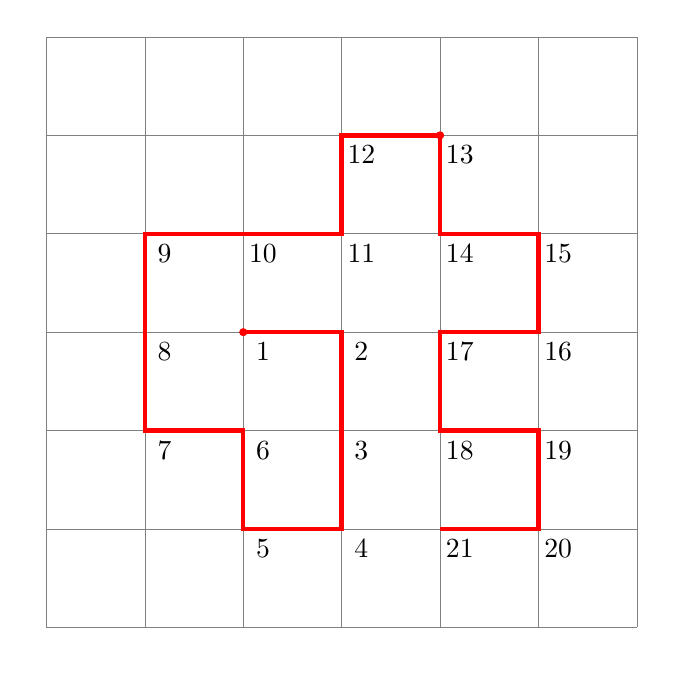
\begin{tikzpicture}[scale=1.25]
% grid
    \foreach \i in {\xMin,...,\xMax} {
        \draw [very thin,gray] (\i,\yMin) -- (\i,\yMax)  node [below] at (\i,\yMin) {};
    }
    \foreach \i in {\yMin,...,\yMax} {
        \draw [very thin,gray] (\xMin,\i) -- (\xMax,\i) node [left] at (\xMin,\i) {};
    }

% start and end of the self avoiding walk
\filldraw[red] (2,3) circle (1pt);
\filldraw[red] (4,5) circle (1pt);

% self avoiding walk
\draw[red, ultra thick] (2,3) -- (3,3) -- (3,2) -- (3,1) -- (2,1) -- (2,2) -- (1,2) -- (1,3) -- (1,4) --
(2,4) -- (3,4) -- (3,5) -- (4,5) -- (4,4) -- (5,4) -- (5,3) -- (4,3) -- (4,2) -- (5,2) --
(5,1) -- (4,1) ;

% self avoiding walk indexing
\node (A) at (2+\xshift,3+\yshift) {1};
\node (B) at (3+\xshift,3+\yshift) {2};
\node (C) at (3+\xshift,2+\yshift) {3};
\node (C) at (3+\xshift,1+\yshift) {4};
\node (D) at (2+\xshift,1+\yshift) {5};
\node (E) at (2+\xshift,2+\yshift) {6};
\node (F) at (1+\xshift,2+\yshift) {7};
\node (G) at (1+\xshift,3+\yshift) {8};
\node (H) at (1+\xshift,4+\yshift) {9};
\node (I) at (2+\xshift,4+\yshift) {10};
\node (J) at (3+\xshift,4+\yshift) {11};
\node (K) at (3+\xshift,5+\yshift) {12};
\node (L) at (4+\xshift,5+\yshift) {13};
\node (M) at (4+\xshift,4+\yshift) {14};
\node (N) at (5+\xshift,4+\yshift) {15};
\node (O) at (5+\xshift,3+\yshift) {16};
\node (P) at (4+\xshift,3+\yshift) {17};
\node (Q) at (4+\xshift,2+\yshift) {18};
\node (R) at (5+\xshift,2+\yshift) {19};
\node (S) at (5+\xshift,1+\yshift) {20};
\node (T) at (4+\xshift,1+\yshift) {21};


\end{tikzpicture} 
 \caption{A self-avoiding walk}
 \label{fig:A self-avoiding walk}
\end{figure}

Fig. \ref{fig:A self-avoiding walk} show a self-avoiding walk in a two dimensional lattice which is a non-self intersecting path on the grid. In the self-avoiding walk, the red line shows the path of the walk. In a two-dimensional lattice, each vertex in a self-avoiding walk can have maximum degree two (except the first and the last vertex which might have three). Similarly in a three-dimensional lattice, each vertex can have a maximum degree of four (the first and the last vertex can have five).

A {\it contact map} is a useful graphical representation(and two-dimensional description ) of the structure of a protein where the vertex set represents the amino acids in the same order in which they appear in the linear sequence of the protein and the edge set represents the set of contacts. In the contact map of a self-avoiding walk, the edges are between vertices which are at a unity distance from each other in the grid but not in the walk.
Fig. \ref{fig:A contact Map Example} shows the contact map of the self avoiding walk shown in Fig. \ref{fig:A self-avoiding walk}.
%The contact map can also be mathematically represented by an $n\times n$ binary matrix. For a protein of
%size $n$, and a given threshold $\mu >0$, the contact map ${M _\mu}$ is an $n\times n$ binary matrix whose entry  ${M _\mu}(i,j)$ equals 1, if the distance between
%two amino acids $i$ and j is less than or equal to $\mu$ or 0 otherwise.
Contact maps of proteins can be used for a wide range of functionality. Few of them are secondary structure prediction, fold identification, fold classification, fold assignment, protein structure alignment and threading \citep{zhang08}. The three-dimensional structure of RNA can also be cast in the form of a contact map and hence this helps in understanding their structure \citep{zhang08}.

\begin{figure}[ht]
\centering
 
\centering
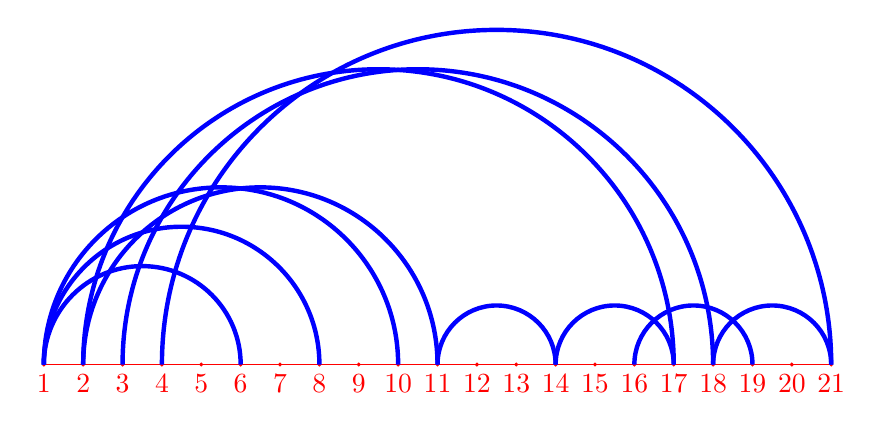
\begin{tikzpicture}[scale=0.5]


\foreach \i in {1,...,20} {
        \draw[red] (\i,1) -- (\i + 1,1)node[pos=0.0,below] {\i};
        \filldraw[red] (\i,1) circle (1pt);


 }

\draw[red] (21,1) -- (20,1)node[pos=0.0,below] {21};
\filldraw[red] (21,1) circle (1pt); 



\draw[blue, ultra thick] (1,1) arc(180:0:2.5); 
\draw[blue, ultra thick] (1,1) arc(180:0:4.5); 
\draw[blue, ultra thick] (1,1) arc(180:0:3.5); 
\draw[blue, ultra thick] (2,1) arc(180:0:4.5);
\draw[blue, ultra thick] (2,1) arc(180:0:7.5);
\draw[blue, ultra thick] (3,1) arc(180:0:7.5);
\draw[blue, ultra thick] (4,1) arc(180:0:8.5);
\draw[blue, ultra thick] (11,1) arc(180:0:1.5);
\draw[blue, ultra thick] (14,1) arc(180:0:1.5);
\draw[blue, ultra thick] (16,1) arc(180:0:1.5);
\draw[blue, ultra thick] (18,1) arc(180:0:1.5);



\end{tikzpicture} 
 \caption{A contact map example}
 \label{fig:A contact Map Example}
\end{figure}
\begin{figure}[ht]
\centering
 
\centering
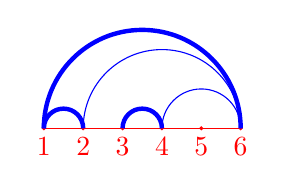
\begin{tikzpicture}[scale=0.5]


\foreach \i in {1,...,5} {
        \draw[red] (\i,1) -- (\i + 1,1)node[pos=0.0,below] {\i};
        \filldraw[red] (\i,1) circle (1pt);


 }

\draw[red] (6,1) -- (5,1)node[pos=0.0,below] {6};
\filldraw[red] (6,1) circle (1pt); 



\draw[blue, ultra thick] (1,1) arc(180:0:0.5); 
\draw[blue, ultra thick] (1,1) arc(180:0:2.5); 
\draw[blue, thin] (2,1) arc(180:0:2);
\draw[blue, ultra thick] (3,1) arc(180:0:0.5);
\draw[blue, thin] (4,1) arc(180:0:1);
\end{tikzpicture} 
 
\centering
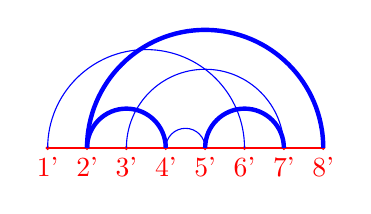
\begin{tikzpicture}[scale=0.5]


\foreach \i in {1,...,7} {
        \draw[red] (\i,1) -- (\i + 1,1)node[pos=0.0,below] {\i'};
        \filldraw[red] (\i,1) circle (1pt);


 }

\draw[red] (8,1) -- (7,1)node[pos=0.0,below] {8'};
\filldraw[red] (8,1) circle (1pt); 



\draw[blue, thin] (1,1) arc(180:0:2.5); 
\draw[blue, ultra thick] (2,1) arc(180:0:1);
\draw[blue, ultra thick] (2,1) arc(180:0:3);
\draw[blue, thin] (3,1) arc(180:0:2);
\draw[blue, thin] (4,1) arc(180:0:0.5);
\draw[blue, ultra thick] (5,1) arc(180:0:1);


\end{tikzpicture} 
\caption{A contact map overlap example}
\label{fig:A contact Map overlap Example}
\end{figure}

Given two contact maps, contact map overlap is defined as the maximum number of contacts preserved by some order-preserving bijection between subsets of the two vertex sets. Let us explain the same with the two contact maps shown in Fig. \ref{fig:A contact Map overlap Example}. The contact overlap between the two graphs is $3$ and these edges are preserved by the order preserving bijection between the two subset of edges $S_1 =\{1,2,3,4,6\}$ of the first graph and $S_2 =\{2^{\prime},4^{\prime},5^{\prime},7^{\prime},8^{\prime}\}$. Using these fundamental concepts, the next section gives a detailed description of the course in which the research has progressed using contact map overlap measure.

The rest of the report is organized as follows. Chapter \ref{approximation} presents the relevant
literature on approximation algorithms for solving the CMO problem.
Chapter \ref{exact} briefly describes some of the exact algorithms proposed
for solving the CMO problem. Finally, Chapter \ref{critique} provides a critical analysis of the
algorithms proposed in Chapter \ref{approximation} and Chapter \ref{exact} and discusses about
possible extensions and research directions. 